% ==============================================================================
%
%                             Scalability
%
% ==============================================================================
\chapter{Scalability} \label{chapt:scalability}
The code for this project is written from the beginning with the possibility to
scale it up in mind. The main idea being that the throughput can be increased.
Scalability in regard to this project can be divided into two terms:
\begin{itemize}
    \item Inside FPGA
    \item Across multiple FPGAs
\end{itemize}

In the following sections these two aspects are dissected theoretically.

\section{Inside FPGA}
Every FPGA has a given amount of ressources (LUTs, memory and so forth, as
described in table \ref{tab:XC7A200T}). The inside FPGA scalability aims towards
optimal usage of these ressources. Before methods for scalability can be
compared it must be clarified what can be scaled. The \gls{diip} project
consists of three main parts. The communication, controller and image processing
parts. The communication part is only implemented once to handle the
communication to the PC and therefore can not be scaled. The image processing
part however can be implemented multiple times inside the FPGA to increase
throughput. Therefore the conrtoller part splits up the incomming image data and
distributes it to the image processing cores. To summarize the inside FPGA
scalability:
\begin{itemize}
    \item Implement the communication part once
    \item Implement the image processing part as many times as the available
    ressources allow it
    \item Adapt the controller to distribute data accross the processing cores
\end{itemize}

Figure \ref{fig:insidefpgascaleconceptbd} clarifies the concept. Note that all
image processing cores are equal.

\begin{figure}[tb!]
    \centering
    \begin{adjustbox}{max width=\linewidth}
        % \tikzsetnextfilename{system-overview}
\begin{tikzpicture}[
    rounded corners=0mm,
]
    %coordinates
    \coordinate (corig)      at (0,0);
    \coordinate (cmonitor)   at (0,0);
    \coordinate (ccom)       at (5,0);
    \coordinate (cip)        at (10,0);


    %nodes

    \begin{pgfonlayer}{main}

        \node[draw, fill=white, minimum width=3cm, minimum height=2cm, anchor=west, text width=2.8cm, align=center] (com) at (ccom) {Controller};

        \node[draw, fill=white, minimum width=3cm, minimum height=1cm, anchor=west, text width=2.8cm, align=center, above =1cm of com] (commu) {Communication};

        \node[draw, fill=white, minimum width=3cm, minimum height=1cm, anchor=west, text width=2.8cm, align=center, right = 1cm of com, yshift=2.5cm] (ip1) {Image\\Processing};
        \node[draw, fill=white, minimum width=3cm, minimum height=1cm, anchor=west, text width=2.8cm, align=center, right = 1cm of com, yshift=1.0cm] (ip2) {Image\\Processing};
        \node[draw, fill=white, minimum width=3cm, minimum height=1cm, anchor=west, text width=2.8cm, align=center, right = 1cm of com, yshift=-0.5cm] (ip3) {Image\\Processing};
        
        \node[circle,fill=black,minimum size=0.2cm,inner sep=0pt, below = 0.3cm of ip3] (dt1)  {};
        \node[circle,fill=black,minimum size=0.2cm,inner sep=0pt, below = 0.2cm of dt1] (dt2)  {};
        \node[circle,fill=black,minimum size=0.2cm,inner sep=0pt, below = 0.2cm of dt2] (dt3)  {};

        % \node[] (eth) at ($(cmonitor) + (4.5, 1.0)$) {LAN};
        
        % \draw[line width = 0.5mm] ($(eth) + (0,-1.0)$) ellipse (0.2cm and 0.5cm);
    \end{pgfonlayer}

    % FPGA box
    \begin{pgfonlayer}{main}
        \node[above = 2.4cm of com, xshift=-1.2cm] (fpga) { FPGA };
    \end{pgfonlayer}
    \begin{pgfonlayer}{foreground}
        \node (f_fpga) [draw=black, fill=gray!20, inner sep=10, fit={(com) (ip1) (ip2) (ip3) (dt2) (dt1) (dt3)}] {};
    \end{pgfonlayer} 

    
    \path[draw,{Latex[length=2.5mm]}-{Latex[length=2.5mm]}] ($(commu.180) + (-1.5,0)$) -- ($(commu.180) + (0,0)$) node[near start, left, anchor=east,xshift=-0.5cm] () {PC} ;
    \path[draw,{Latex[length=2.5mm]}-{Latex[length=2.5mm]}] ($(com.90) + (0,0)$) -- ($(commu.270) + (0,0)$) node[near start, left, anchor=east,xshift=-0.5cm] () {} ;

    \path[draw,{Latex[length=2.5mm]}-{Latex[length=2.5mm]}] 
        ($(com.0) + (0,0.7)$) -| ($(ip1.180) + (-0.6,0)$) -- ($(ip1.180) + (0,0)$)
         node[near start, left, anchor=east,xshift=-0.5cm] () {} ;
    \path[draw,{Latex[length=2.5mm]}-{Latex[length=2.5mm]}] 
        ($(com.0) + (0,0.1)$) -| ($(ip2.180) + (-0.4,0)$) -- ($(ip2.180) + (0,0)$) 
        node[near start, left, anchor=east,xshift=-0.5cm] () {} ;
    \path[draw,{Latex[length=2.5mm]}-{Latex[length=2.5mm]}] ($(com.0) + (0,-0.5)$) -- ($(ip3.180) + (0,0)$) node[near start, left, anchor=east,xshift=-0.5cm] () {} ;


\end{tikzpicture}
    \end{adjustbox}
    \caption{Block diagram of a inside FPGA scaled solution}
    \label{fig:insidefpgascaleconceptbd}
\end{figure}

Now that the concept is clarified, two possible solutions are compared to
distribute the image data accross the image processing cores, proposal A and B.
They differ in the way in what order the data is sent to the FPGA and how it is
cached inside the FPGA. For each proposal the following metrics are calculated.

\begin{description}
    \item[Initial size $s_i$]\hfill \\
    The number of pixels that have to be sent to the FPGA before beginning
    interational operation.
    \item[Iteration size $s_r$]\hfill \\
    How many pixels that have to be sent to start a new iteration.
    \item[Store size $s_s$]\hfill \\
    How many pixels have to be cached inside the FPGA.
    \item[Number of inits per image $n_i$]\hfill \\
    Denotes the number of initial data transfers of size $s_i$ have to be made
    per image.
    \item[Total tx size $s_{tx}$]\hfill \\
    The total number of pixels sent to the FPGA to calculate one image.
    \item[Number of image processing cores $N$]\hfill \\
    The number of image processing cores implemented on the FPGA.
\end{description}


\begin{table}[tb!]
    \centering
    \begin{tabular}{p{0.45\textwidth} p{0.45\textwidth}}
        \toprule
        \multicolumn{1}{c}{Proposal A} & \multicolumn{1}{c}{Proposal B} \\
        \midrule
            \begin{adjustbox}{max width=0.4\textwidth}
                \input{images/scalability/proposela.tikz}
            \end{adjustbox}
        & 
            \begin{adjustbox}{max width=0.4\textwidth}
                % \tikzsetnextfilename{system-overview}
\begin{tikzpicture}[
    rounded corners=0mm,
    triangle/.style = {fill=blue!20, regular polygon, regular polygon sides=3 },
    node rotated/.style = {rotate=180},
    border rotated/.style = {shape border rotate=180}
]
    %coordinates
    \coordinate (orig)      at (0,0);

    \begin{pgfonlayer}{main}
        
        % Braces
        \draw [line width=0.5mm,decorate,decoration={brace,amplitude=10pt},xshift=-4pt,yshift=0pt] (9.5,7) -- (9.5,3) node [black,midway,xshift=0.5cm,anchor=north,rotate=90] {$w_l+(N-1)$};
        % \draw [line width=0.5mm,decorate,decoration={brace,amplitude=10pt},xshift=-0pt,yshift=0pt] (8,-0.5) -- (0,-0.5) node [black,midway,yshift=-0.5cm,anchor=north] {Image width};
        
        % Center pixel
        % \draw[black,line width=0.5mm] (2,2) rectangle (3,3);
        
        % Window sizes
        \draw[blue,line width=0.6mm] (0,4) rectangle (3,7);
        \draw[red,line width=0.6mm,dashed] (0,3) rectangle (3,6);
        % \draw[black,line width=0.6mm,dotted] (0,2) rectangle (3,5);
        % resulting lines
        \draw[cyan,line width=0.6mm] (1,5) rectangle (8,6);
        \draw[magenta,line width=0.6mm,dashed] (1,4) rectangle (8,5);
        % \draw[black,line width=0.3mm,dotted] (1,3) rectangle (5,4);

        % Arrows
        % \path[draw,-{Latex[length=2.5mm]},line width=0.4mm] (0,7.5) -- (4,7.5) 
        %     node[near start, above] () {send data} ;
        % \path[draw,-{Latex[length=3.5mm]},line width=0.4mm] (-0.5,7) -- (-0.5,3) 
        %     node[near start, above,rotate=270] () {init} ;

        % Axis
        \foreach \y in {0,1,2,3,4,5,6}
            \node[anchor=west] at ($(-0.5,6.5)-(0,\y)$)  {$\y$};
        \foreach \x in {0,1,2,3,4,5,6,7,8}
            \node[anchor=north] at ($(0.5,7.5)+(\x,0)$)  {$\x$};

        % out pixels
        \foreach \x in {0,1,2,3,4,5,6}
            \node[anchor=center] at ($(1.5,5.5)+(\x,0)$)  {$\x_{c0}$};
        \foreach \x in {0,1,2,3,4,5,6}
            \node[anchor=center] at ($(1.5,4.5)+(\x,0)$)  {$\x_{c1}$};


    \end{pgfonlayer}

    % Foreground
    \begin{pgfonlayer}{foreground}
        
    \end{pgfonlayer} 

    % Background
    \begin{pgfonlayer}{background}
        % Init pixels
        \draw[fill=gray!20] (0,3) rectangle (3,7);
        % Iter pixels
        \draw[pattern=north east lines, pattern color=gray!60] (3,3) rectangle (4,7);
        % Grid
        \draw[step=1cm,black,thin] (0,0) grid (9,7);
    \end{pgfonlayer} 

\end{tikzpicture}
            \end{adjustbox}
        \\
        % \multicolumn{1}{c}{caption}&
        % \multicolumn{1}{c}{caption}
        % \\
        \multicolumn{2}{c}{
            \begin{adjustbox}{max width=0.8\textwidth}
                % \tikzsetnextfilename{system-overview}
\begin{tikzpicture}[
    rounded corners=0mm,
    triangle/.style = {fill=blue!20, regular polygon, regular polygon sides=3 },
    node rotated/.style = {rotate=180},
    border rotated/.style = {shape border rotate=180}
]
    %coordinates
    \coordinate (orig)      at (0,0);

    \begin{pgfonlayer}{main}
        
        % Init pixels
        \draw[fill=gray!20] (0,0) rectangle (1,0.6);
        \node[anchor=west] at (1.2,0.3)  {Init data};

        \draw[pattern=north east lines, pattern color=gray!60] (3,0) rectangle (4,0.6);
        \node[anchor=west] at (4.2,0.3)  {Iteration data};

        \draw[blue,line width=0.6mm] (7,0) rectangle (8,0.6);
        \draw[red,line width=0.6mm,dashed] (8.5,0) rectangle (9.5,0.6);
        % \draw[black,line width=0.4mm,dotted] (10,0) rectangle (11,0.6);
        \node[anchor=west] at (9.7,0.3)  {Image processing cores};
        % Iter pixels
        % \draw[pattern=north east lines, pattern color=gray!60] (3,2) rectangle (4,7);
    \end{pgfonlayer}

    % Foreground
    \begin{pgfonlayer}{foreground}
        
    \end{pgfonlayer} 

    % Background
    \begin{pgfonlayer}{background}
        % Grid
        % \draw[step=1cm,gray,thin] (0,0) grid (6,7);
    \end{pgfonlayer} 

\end{tikzpicture}
            \end{adjustbox}
        }
        \\\midrule
        \textbf{Concept} & \\
        Image data is sent line wise. Each image processing core handles one
        input line, starts as soon as enough data is transfered and jumps $N$ lines
        downwards after completion.
        &
        Image data is sent coloumn wise with $w_l+(N-1)$ pixels per coloumn. All
        image processing cores start processing at the same time and progress
        $N$ lines downwards after completion.
        \\\midrule
        \textbf{Initial size} & \\
        {\( 
            s_i = i_w(w_l+(N-1))
        \)}
        &
        {\( 
            s_i = w_l(w_l+(N-1))
        \)}
        \\\midrule
        \textbf{Iterarion size} & \\
        {\( 
            s_r  = i_w
        \)}
        &
        {\( 
            s_r  = w_l+(N-1)
        \)}
        \\\midrule
        \textbf{Store size} & \\
        {\( 
            s_s  = i_w(w_l+(N-1))
        \)}
        &
        {\( 
            s_s  = w_l(w_l+(N-1))
        \)}
        \\\midrule
        \textbf{Number of inits per image} & \\
        {\( 
            n_i  = 1
        \)}
        &
        {\( 
            n_i  = \frac{1}{N}(i_w-w_l+1)
        \)}
        \\\midrule
        \textbf{Total tx size} & \\
        {\( 
            s_{tx}  = i_w \cdot i_h
        \)}
        &
        {\( 
            s_{tx}  = n_i s_i + (i_w-w_l)s_r n_i
        \)}
        \\
        \bottomrule
    \end{tabular}
    \caption{Inside FPGA scalability proposals}
    \label{tab:insidefpgascalability}
\end{table}

Before comparing the two proposals another metric has to be taken into
consideration: The effective throughput of the image processing core. The way
the wallis filter works is that it requires a neighbourhood of pixels. For each
line the core processes, the initial neighbourhood has to be sent. Equation
\ref{eq:theomaxvhdlwallise} derived in appendix 
\ref{app:derivations:theomaxvhdlwallis} is used to calculate the effective
throughput $b_r$ of a Wallis filter core. To simplify, the image height $i_h$ is
considered to be much larger than the window length $w_l$ and therefore the
equation can be noted as shown in equation \ref{eq:vhdlwallismaxb}. Using the
throughput of the VHDL Wallis filter implementation ($b_w=125Mp/s$) and the
window length $w_l=21$ the effective bandwidth $b_r$ is calculated:

\begin{align}
    b_r  & \approx \frac{b_w}{w_l} = 5.95 Mp/s
    \label{eq:vhdlwallismaxb}
\end{align}

Under the assumption that the real throughput $b_r$ scales proportionally with the
number of image processing cores implemented, equation 
\ref{eq:scaledrealttotalhroughput} can be noted to represent the total image
processing throughput $b_t$.

\begin{align}
    b_t  & = N \cdot b_r
    \label{eq:scaledrealttotalhroughput}
\end{align}

Considering the maximum throughput of the Gigabit-Ethernet connection of
$b_e=125MB/s$ \footnote{True Ethernet throughput is less than 125MB/s
considering packet overhead} equation \ref{eq:maxethernetthrouhgput} can be derived to calculate the
maximum number of image processing cores that can be implemented before the
Ethernet communication link is saturated.

\begin{align}
    b_e \geq b_t = N \cdot b_r \Rightarrow N \leq \frac{b_e}{b_r} \approx 
    \frac{b_e w_l}{b_w} = w_l = 21
    \label{eq:maxethernetthrouhgput}
\end{align}

To calculate the free memory the results from \ref{asdf} \todo{ref to ressource
VHDL} are dissected to calculate the available memory. Table \ref{tab:membudget}
lists the required block memory usage.

\begin{table}[h!]
    \centering
    \begin{tabular}{l r}
        \toprule
        Item & BRAM tiles \\
        \midrule
        Total available & 365 \\
        TEMAC support & -2 \\
        UDP IP Core & -1.5 \\
        21 divider generators & -10.5 \\
        21 Wallis cores & -10.5 \\
        \midrule
        Free & 340.5\\
        \bottomrule
    \end{tabular}
    \caption{FPGA block memory budget}
    \label{tab:membudget}
\end{table}

After using up memory for the communication and image processing cores, 340.5
block RAM tiles with 36Kb each results in 1'496KB of remaining block RAM that
can be used for image caching. Table \ref{tab:parsum} summarizes the
parameters that are used to compare the two inside FPGA scale proposals.

\begin{table}[h!]
    \centering
    \begin{tabular}{l r l}
        \toprule
        Parameter & Value & Description\\
        \midrule
        $N$ & 21 & Number of image processing cores to implement \\
        $s_b$ & 1'532KB & Block memory storage available for cache \\
        $w_l$ & 21 & Window length of the Wallis filter \\
        \bottomrule
    \end{tabular}
    \caption{Parameter summary}
    \label{tab:parsum}
\end{table}

Now the two proposals can be put to contrast. Starting with figure 
\ref{fig:sca:compfixheight} the two proposals are compared against each other
with an input image of fixed height and variable with. This was chosen because
with the main limiting factor being \gls{bramtile} usage, the store size $s_s$ has to
be observed and it is for both proposals independant of image height $i_h$. The
two proposals can be differentiated in that proposal A is optimized for low tx
size $s_{tx}$ (and therefore optimized for throughput) while proposal B requires
buch less memory (area optimized). 
\\
The BRAM usage is best utilized by proposal A at approximately
$i_w=32Kp$\footnote{32 is chosen because it is a power of two} while
the necessary tx size is kept at the minimum. Its one disatvantage being the
limited image width of 32Kp. Three workarounds can be considered to raise the
limit in image width:
\begin{itemize}
    \item Use less image processing cores. This would decrease the required
    block memory and the image width can be increased. However by decreasing the
    number of image processing cores, the total throughput would also drop.
    \item Use proposal B. Its BRAM usage is significantly smaller however the tx
    size will increase.
    \item Split the image on the PC and process each coloumn as if it was a
    single image.
\end{itemize}

This problem leads to the next term in scalability: The scalability across
multiple FPGA.

\begin{figure}[tb!]
    \centering
    \begin{adjustbox}{max width=\linewidth}
        % Preamble: 
% \pgfplotsset{width=7cm,compat=1.5.1}
\begin{adjustbox}{max width=1\linewidth}
\begin{tabular}{c c}
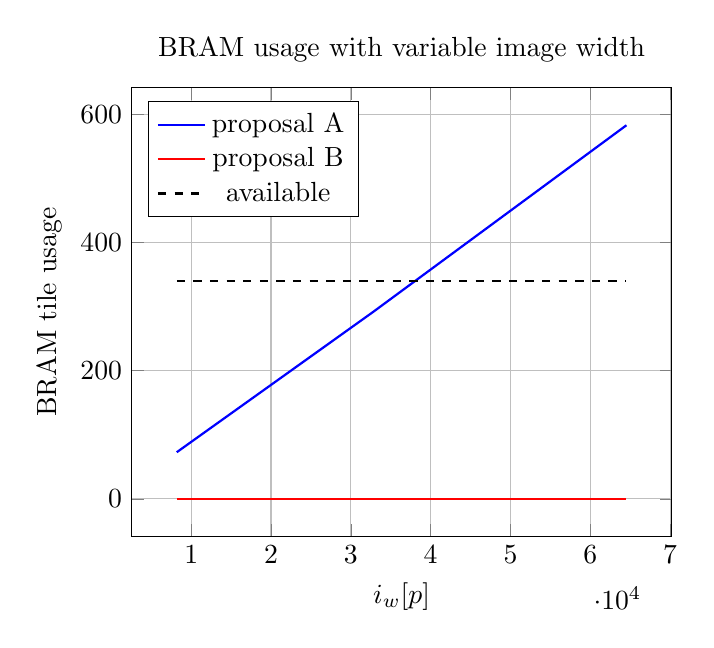
\begin{tikzpicture}
    % \pgfplotsset{
    %     scaled x ticks=base 10:3
    % }
    \begin{axis}[
            % height=9cm,
            % width=9cm,
            grid=major,
            title=BRAM usage with variable image width,
            xlabel=$i_w \lbrack p \rbrack$,
            ylabel=BRAM tile usage,
            legend pos=north west,
            % xtick={10,20,...,70},
            every axis plot/.append style={thick}
        ]

            \addplot[mark=none,blue] coordinates {
                (8192, 72.88888889)
                (16384,145.7777778)
                (32768,291.5555556)
                (64536,583.1111111)
            };
            \addlegendentry{proposal A}

            \addplot[mark=none,red] coordinates {
                (8192, 0.186848958)
                (16384,0.186848958)
                (32768,0.186848958)
                (64536,0.186848958)
            };
            \addlegendentry{proposal B}
            
            \addplot[mark=none, black, dashed] coordinates {(8192,340.5) (64536,340.5)};
            \addlegendentry{available}
    \end{axis}
\end{tikzpicture}
&
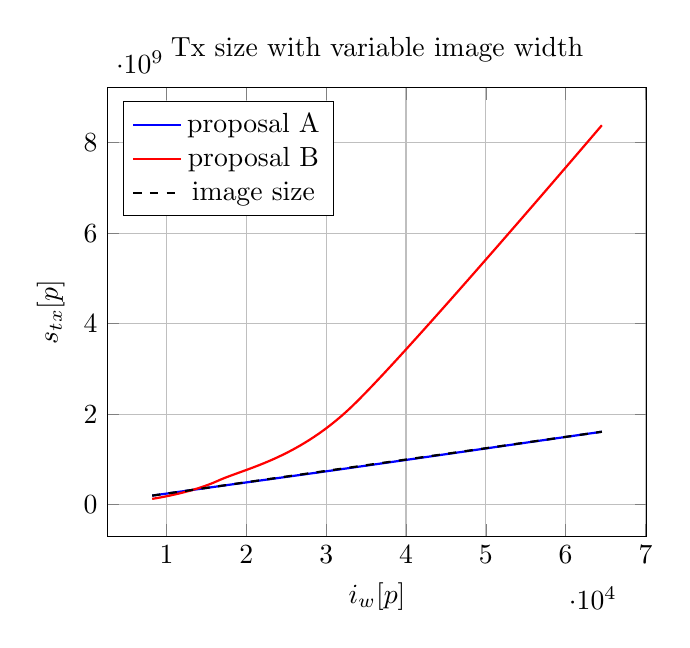
\begin{tikzpicture}
    \begin{axis}[
            % height=9cm,
            % width=9cm,
            grid=major,
            title=Tx size with variable image width,
            xlabel=$i_w \lbrack p \rbrack$,
            ylabel=$s_{tx} \lbrack p \rbrack$,
            legend pos=north west,
            % xtick={10,20,...,70},
            every axis plot/.append style={thick}
        ]

            \addplot[mark=none,blue,smooth] coordinates {
                (8192, 198967296)
                (16384, 402653184)
                (32768, 805306368)
                (64536, 1610612736)
            };
            \addlegendentry{proposal A}

            \addplot[mark=none,red,smooth] coordinates {
                (8192, 127795360)
                (16384, 523288576)
                (32768, 2094497792)
                (64536, 8383365120)
            };
            \addlegendentry{proposal B}
            
            \addplot[mark=none, black, dashed] coordinates {(8192,198967296) (64536,1610612736)};
            \addlegendentry{image size}
    \end{axis}
\end{tikzpicture}
\end{tabular}
\end{adjustbox}

    \end{adjustbox}
    \caption{Comparing proposals width variable image width ($w_l=N=21$,
    $i_h=24'576$)}
    \label{fig:sca:compfixheight}
\end{figure}


\section{Across FPGA}
Now that one FPGA is capable of processing image data at the rate at which it is
trasfered to it through Ethernet, the solution can be scaled on a network. This
was the main reason to use Ethernet as communication basis. An input image is
split into parts on the computer and processed individually by FPGAs. The
processed pixels are merged together on the PC to form the output image. Figure
\ref{fig:sca:acrossfpgapart} illustrates a coloumn wise image splitting to three
parts. The colored boxes represent one Wallis filter processing a single line.

\begin{figure}[tb!]
    \centering
    \begin{adjustbox}{max width=\linewidth}
        % \tikzsetnextfilename{system-overview}
\begin{tikzpicture}[
    rounded corners=0mm,
    triangle/.style = {fill=blue!20, regular polygon, regular polygon sides=3 },
    node rotated/.style = {rotate=180},
    border rotated/.style = {shape border rotate=180}
]
    %coordinates
    \coordinate (orig)      at (0,0);

    \begin{pgfonlayer}{main}
        
        % Braces
        \draw [line width=0.5mm,decorate,decoration={brace,amplitude=10pt},xshift=-4pt,yshift=0pt] (12.5,4) -- (12.5,0) node [black,midway,xshift=0.5cm,anchor=west] {$i_h$};
        \draw [line width=0.5mm,decorate,decoration={brace,amplitude=10pt},xshift=-0pt,yshift=0pt] (12,-0.3) -- (0,-0.3) node [black,midway,yshift=-0.5cm,anchor=north] {$i_w$};
        
        % Center pixel
        % \draw[black,line width=0.5mm] (2,2) rectangle (3,3);
        
        % Window sizes
        \draw[blue,line width=0.6mm] (0,3) rectangle (4.5,4);
        \draw[red,line width=0.6mm] (3.5,3) rectangle (8.5,4);
        \draw[green,line width=0.6mm] (7.5,3) rectangle (12,4);
        % \draw[black,line width=0.6mm,dotted] (0,2) rectangle (3,5);

        % Meas lines
        \path[draw,-] (3.5,4) -- (3.5,4.8);
        \path[draw,-] (4.0,4) -- (4.0,4.8);
        \path[draw,-{Latex[length=2.5mm]}] (3,4.5) -- (3.5,4.5);
        \path[draw,-] (3.5,4.5) -- (4.0,4.5);
        \path[draw,-{Latex[length=2.5mm]}] (5,4.5) -- (4.0,4.5) 
            node[near start, anchor=south west] {$\lfloor \frac{w_l}{2} \rfloor$};
        % Arrows
        % \path[draw,-{Latex[length=2.5mm]}] (0,7.5) -- (4,7.5) 
        %     node[near start, above] () {iterate} ;
        % \path[draw,-{Latex[length=3.5mm]},line width=0.4mm] (-0.5,7) -- (-0.5,3) 
        %     node[near start, above,rotate=270] () {iterate} ;

        % Axis
        % \foreach \x in {0,1,2,3,4}
        %     \node[anchor=north] at ($(-0.5,5)-(0,\x)$)  {$\x$};

        \node[anchor=center] at (2,2) {FPGA 1};
        \node[anchor=center] at (6,2) {FPGA 2};
        \node[anchor=center] at (10,2) {FPGA 3};

    \end{pgfonlayer}

    % Foreground
    \begin{pgfonlayer}{foreground}
        
    \end{pgfonlayer} 

    % Background
    \begin{pgfonlayer}{background}
        % resulting lines
        \draw[blue,line width=0.3mm,fill=blue!20] (0.5,3.4) rectangle (4,3.6);
        \draw[red,line width=0.3mm,fill=red!20] (4,3.4) rectangle (8,3.6);
        \draw[green,line width=0.3mm,fill=green!20] (8,3.4) rectangle (11.5,3.6);
        % % Init pixels
        % \draw[fill=gray!20] (0,3) rectangle (6,7);
        % % Iter pixels
        % \draw[pattern=north east lines, pattern color=gray!60] (0,2) rectangle (6,3);
        % Grid
        \draw[step=4cm,black] (0,0) grid (12,4);
    \end{pgfonlayer} 

\end{tikzpicture}
    \end{adjustbox}
    \caption{Image partitioning for distribution across multiple FPGA}
    \label{fig:sca:acrossfpgapart}
\end{figure}

For the Wallis filter operation, the image data has to be overlapped between the
segments to omit the loss of pixels where the image is cut. To calculate the
throughput of a distributed FPGA image processing solution, this multiple
sending of data has to be taken into consideration. Equation 
\ref{eq:sca:linesize} derives how the total line size $s_l$ is calculated in
reference to the number of FPGAs $N_F$ the image is distributed to. Width the
image width $i_w$ being much greater than the window length $w_l$, 
\ref{eq:sca:linesize} can be approximated.

\begin{align}
    s_l  & = i_w & (N_f = 1) \\
         & = i_w + (N_F-1) \cdot 2 \cdot \lfloor\frac{w_l}{2}\rfloor & \\
         & = i_w + (N_F-1)(w_l-1) & (w_l=2k+1, k \in \mathbb{N} )\\
         & \approx i_w & (i_w \gg w_l)
    \label{eq:sca:linesize}
\end{align}

Concluding this finding it can be infered that the throughput of a distributed
image processing solution scales proportionally to the number of FPGAs the image
is distributed to:
\begin{align}
    b_t & \propto N_F \\
        & \approx N_F \cdot b_e
\end{align}
\begin{tabular}{rl}
    $b_t        =$ & Total throughput of distributed image processing \\
    $N_F        =$ & Number of FPGAs used \\
    $b_e        =$ & Throughput of Ethernet connection to the FPGA \\
\end{tabular} \\

A last thought is put on the network infrastructure that is required to
process iamges distributed. The network link of 1Gb/s on the FPGA's Ethernet
port is saturated. Therefore if multiple FPGAs are used on a network, the
interconnecting network switch must be capable of an uplink to the PC or server
with a multiple of the throughput of the FPGA downlink. Figure 
\ref{fig:sca:network} illustrates a network where 10 FPGAs are connected to a
gigabit switch that features an uplink port supporting 10Gb/s throughput. An
example would be the GS418TPP switch \cite{netgearswitch}. 16 gigabit ports
could be used to connect to FPGAs and the SFP uplink port using fibre or copper
to connect to a PC.

\begin{figure}[tb!]
    \centering
    \begin{adjustbox}{max width=\linewidth}
        % \tikzsetnextfilename{system-overview}
\begin{tikzpicture}[
    rounded corners=0mm,
]
    %coordinates
    \coordinate (orig)   at (0,0);
    \coordinate (l)    at (0,0);
    \coordinate (c)    at (4,0);
    \coordinate (tc)    at (4,2);
    \coordinate (r)    at (8,0);

    %nodes
    \node[draw, minimum width=2cm, minimum height=1cm, anchor=south, text width=2cm, align=center] (A) at (l) {PC};
    \node[draw, minimum width=2cm, minimum height=1cm, anchor=south, text width=2cm, align=center] (B) at (c) {FPGA 1};
    \node[draw, minimum width=2cm, minimum height=1cm, anchor=south, text width=2cm, align=center] (C) at (r) {FPGA 2};
    \node[draw, minimum width=2cm, minimum height=1cm, anchor=south, text width=2cm, align=center] (D) at (tc) {Switch};
    
    \path[draw,{Latex[length=2.5mm]}-{Latex[length=2.5mm]}] (A) |- ($(A)!1/2!(A |- D)$) coordinate (xx) -| ($(D.270) + (-1/2,0)$) ;
    \path[draw,{Latex[length=2.5mm]}-{Latex[length=2.5mm]}] (B) |- ($(B)!1/2!(B |- D)$) coordinate (xx) -| ($(D.270) + (0,0)$);
    \path[draw,{Latex[length=2.5mm]}-{Latex[length=2.5mm]}] (C) |- ($(C)!1/2!(C |- D)$) coordinate (xx) -| ($(D.270) + (1/2,0)$);
  
\end{tikzpicture}
    \end{adjustbox}
    \caption{Network topology required to distribute workload onto multiple
    FPGAa}
    \label{fig:sca:network}
\end{figure}

\section{Conclusion}
By scaling the Wallis filter operation inside the FPGA full advantage can be
taken of the available Ethernet bandwith. The controller core thereby caches as
many input lines as can be fitted into block memory to reduce multiple
transmissions of image data and increasing link efficiency. By dividing the input
image into multiple coloumns it can be distributed onto multiple FPGAs on a
network. This scalability across FPGAs is only limited by the network
infrastructure.
\\

Assuming the VHDL implementation of the Wallis filter is used as image
processing core, it can be scaled 21 times inside the FPGA before the Ethernet
communication link is saturated. Using a 10Gb/s switch and and 10 FPGAs a total
image processing throughput of $b_t=10*1Gb/s=1.25GB/s$ can be achieved.


